%%%%%%%%%%%%%%%%%%%%%%%%%%%%%%%%%%%%%%%%%%%%%%%%%%%%%%%%%%%%%%%%%%%%%
%% This is a (brief) model paper using the achemso class
%% The document class accepts keyval options, which should include
%% the target journal and optionally the manuscript type. 
%%%%%%%%%%%%%%%%%%%%%%%%%%%%%%%%%%%%%%%%%%%%%%%%%%%%%%%%%%%%%%%%%%%%%
\documentclass[journal=jacsat,manuscript=article]{achemso}

%%%%%%%%%%%%%%%%%%%%%%%%%%%%%%%%%%%%%%%%%%%%%%%%%%%%%%%%%%%%%%%%%%%%%
%% Place any additional packages needed here.  Only include packages
%% which are essential, to avoid problems later. Do NOT use any
%% packages which require e-TeX (for example etoolbox): the e-TeX
%% extensions are not currently available on the ACS conversion
%% servers.
%%%%%%%%%%%%%%%%%%%%%%%%%%%%%%%%%%%%%%%%%%%%%%%%%%%%%%%%%%%%%%%%%%%%%
\usepackage[version=3]{mhchem} % Formula subscripts using \ce{}
\usepackage{algorithm}
\usepackage{algpseudocode}
\usepackage{svg}
\usepackage{amsmath}
\usepackage{hyperref}

%%%%%%%%%%%%%%%%%%%%%%%%%%%%%%%%%%%%%%%%%%%%%%%%%%%%%%%%%%%%%%%%%%%%%https://www.overleaf.com/project/63f3627b7f8554c152639004
%% If issues arise when submitting your manuscript, you may want to
%% un-comment the next line.  This provides information on the
%% version of every file you have used.
%%%%%%%%%%%%%%%%%%%%%%%%%%%%%%%%%%%%%%%%%%%%%%%%%%%%%%%%%%%%%%%%%%%%%
%%\listfiles

%%%%%%%%%%%%%%%%%%%%%%%%%%%%%%%%%%%%%%%%%%%%%%%%%%%%%%%%%%%%%%%%%%%%%
%% Place any additional macros here.  Please use \newcommand* where
%% possible, and avoid layout-changing macros (which are not used
%% when typesetting).
%%%%%%%%%%%%%%%%%%%%%%%%%%%%%%%%%%%%%%%%%%%%%%%%%%%%%%%%%%%%%%%%%%%%%
\newcommand*\mycommand[1]{\texttt{\emph{#1}}}

%%%%%%%%%%%%%%%%%%%%%%%%%%%%%%%%%%%%%%%%%%%%%%%%%%%%%%%%%%%%%%%%%%%%%
%% Meta-data block
%% ---------------
%% Each author should be given as a separate \author command.
%%
%% Corresponding authors should have an e-mail given after the author
%% name as an \email command. Phone and fax numbers can be given
%% using \phone and \fax, respectively; this information is optional.
%%
%% The affiliation of authors is given after the authors; each
%% \affiliation command applies to all preceding authors not already
%% assigned an affiliation.
%%
%% The affiliation takes an option argument for the short name.  This
%% will typically be something like "University of Somewhere".
%%
%% The \altaffiliation macro should be used for new address, etc.
%% On the other hand, \alsoaffiliation is used on a per author basis
%% when authors are associated with multiple institutions.
%%%%%%%%%%%%%%%%%%%%%%%%%%%%%%%%%%%%%%%%%%%%%%%%%%%%%%%%%%%%%%%%%%%%%
\author{Nicholas Runcie}
\altaffiliation{EaSTCHEM School of Chemistry, University of Edinburgh, EH9 3FJ}
\author{Antonia S.J.S. Mey}
\altaffiliation{EaSTCHEM School of Chemistry, University of Edinburgh, EH9 3FJ}
\email{antonia.mey@ed.ac.uk}
\phone{xxx}


%%%%%%%%%%%%%%%%%%%%%%%%%%%%%%%%%%%%%%%%%%%%%%%%%%%%%%%%%%%%%%%%%%%%%
%% The document title should be given as usual. Some journals require
%% a running title from the author: this should be supplied as an
%% optional argument to \title.
%%%%%%%%%%%%%%%%%%%%%%%%%%%%%%%%%%%%%%%%%%%%%%%%%%%%%%%%%%%%%%%%%%%%%
\title[SILVR: Molecular Generation for binding modes]
  {SILVR: Conditional diffusion model for molecule generation without additional training}
\title[SILVR: Molecular Generation for binding modes]
  {SILVR:Directed Diffusion for Molecule Generation}
%%%%%%%%%%%%%%%%%%%%%%%%%%%%%%%%%%%%%%%%%%%%%%%%%%%%%%%%%%%%%%%%%%%%%
%% Some journals require a list of abbreviations or keywords to be
%% supplied. These should be set up here, and will be printed after
%% the title and author information, if needed.
%%%%%%%%%%%%%%%%%%%%%%%%%%%%%%%%%%%%%%%%%%%%%%%%%%%%%%%%%%%%%%%%%%%%%
\abbreviations{}
\keywords{ML, generative models, docking}

%%%%%%%%%%%%%%%%%%%%%%%%%%%%%%%%%%%%%%%%%%%%%%%%%%%%%%%%%%%%%%%%%%%%%
%% The manuscript does not need to include \maketitle, which is
%% executed automatically.
%%%%%%%%%%%%%%%%%%%%%%%%%%%%%%%%%%%%%%%%%%%%%%%%%%%%%%%%%%%%%%%%%%%%%
\begin{document}

%%%%%%%%%%%%%%%%%%%%%%%%%%%%%%%%%%%%%%%%%%%%%%%%%%%%%%%%%%%%%%%%%%%%%
%% The "tocentry" environment can be used to create an entry for the
%% graphical table of contents. It is given here as some journals
%% require that it is printed as part of the abstract page. It will
%% be automatically moved as appropriate.
%%%%%%%%%%%%%%%%%%%%%%%%%%%%%%%%%%%%%%%%%%%%%%%%%%%%%%%%%%%%%%%%%%%%%
\begin{tocentry}

Some journals require a graphical entry for the Table of Contents.
This should be laid out ``print ready'' so that the sizing of the
text is correct.

Inside the \texttt{tocentry} environment, the font used is Helvetica
8\,pt, as required by \emph{Journal of the American Chemical
Society}.

The surrounding frame is 9\,cm by 3.5\,cm, which is the maximum
permitted for  \emph{Journal of the American Chemical Society}
graphical table of content entries. The box will not resize if the
content is too big: instead it will overflow the edge of the box.

This box and the associated title will always be printed on a
separate page at the end of the document.

\end{tocentry}

%%%%%%%%%%%%%%%%%%%%%%%%%%%%%%%%%%%%%%%%%%%%%%%%%%%%%%%%%%%%%%%%%%%%%
%% The abstract environment will automatically gobble the contents
%% if an abstract is not used by the target journal.
%%%%%%%%%%%%%%%%%%%%%%%%%%%%%%%%%%%%%%%%%%%%%%%%%%%%%%%%%%%%%%%%%%%%%
\begin{abstract}
I'll be an abstract when I grow up. 
\end{abstract}

%%%%%%%%%%%%%%%%%%%%%%%%%%%%%%%%%%%%%%%%%%%%%%%%%%%%%%%%%%%%%%%%%%%%%
%% Start the main part of the manuscript here.
%%%%%%%%%%%%%%%%%%%%%%%%%%%%%%%%%%%%%%%%%%%%%%%%%%%%%%%%%%%%%%%%%%%%%
\section{Introduction}
\label{sec:intro}
One of the challenges as part of computer aided drug-design is to sample from the very large space of possible drug-like compounds to find suitable hits for a given target protein. It is estimated that there are between $10^23$ to $10^60$ possibly feasible compounds, while only around $10^8$ have been synthesised so far~\cite{polishchuk2013estimation, reymond2012exploring}. Different strategies have been employed in the past to try and sample a diverse and synthetically accessible molecular space. In particular, methods based on machine-learning have shown vast amount of promise in recent years in this space~\cite{bilodeau2022generative}. Various different neural network architectures have been proposed for molecular generation, from Varational autoencoders (VAE)~\cite{kingma2022autoencoding, jin2018junction, ma2018constrained}, to generative adversarial networks (GAN)~\cite{hoffmann2019generating} and normalising flows~\cite{shi2021learning}. More recently denoising difusion probailistic models, and particularly equivarient diffusion models have shown promise in moleculear generation~\cite{xu2022geodiff, hoogeboom2022equivariant}.  

- Model generation isn't everything
- How do models fit into hit design, conditioned training needed.


Linker learning with reinforcement learning~\cite{guo2023linkinvent}.

- Equivariant diffusion models have been very promising in predicting 3D structures of drug-like molecules. 
- This does not make them suitable candidates for a target binding site. 
- We combine equivariant diffusion models~\cite{huang2022mdm} with Iterative latent variable refinement proposed in Denoising Diffusion probabilistic models~\cite{choi2021ilvr}.
- This allows the generation of new molecules in the shape of the binding site using information from existing fragments.
\begin{figure}
    \centering
    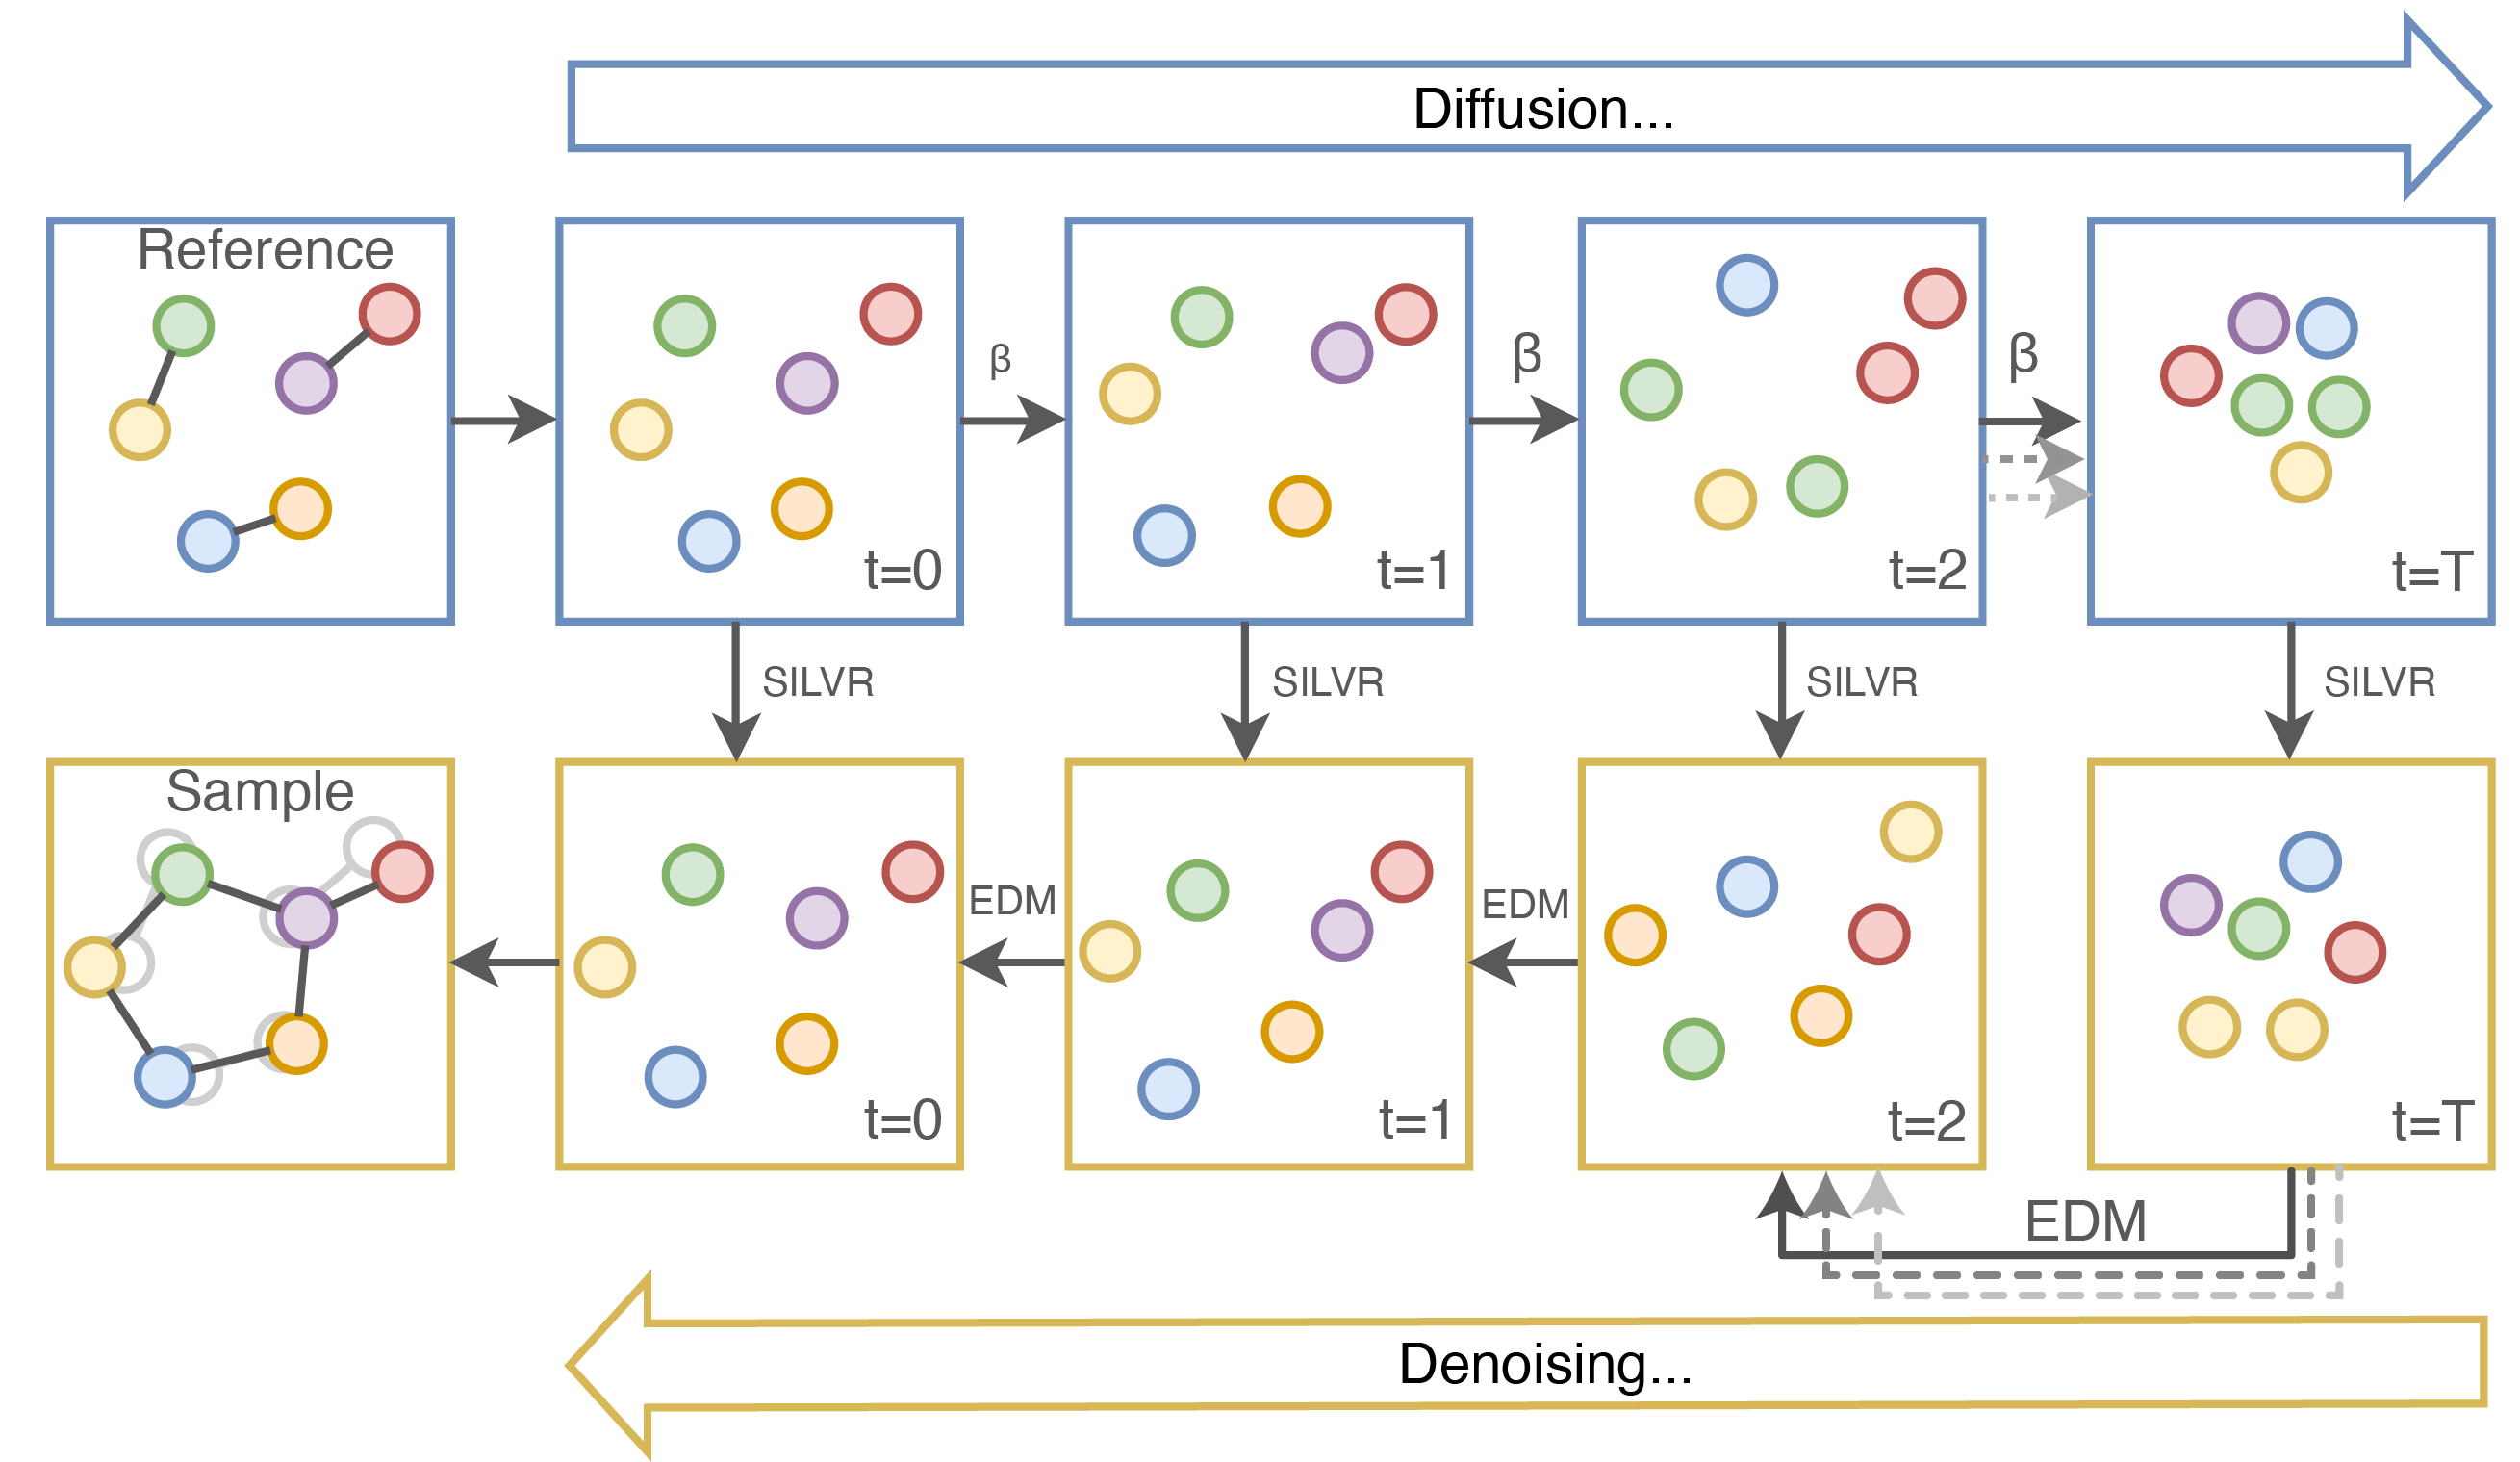
\includegraphics[width=\textwidth]{paper/Figures/Fig1/Schematic.png}
    \caption{Schematic of the equivariant diffusion model with  SILVR indicated for every denoising step.}
    \label{fig:schematic}
\end{figure}
\section{Theory}
\label{sec:theory}
\subsection*{Denoising Diffusion probabilistic models (DDPM) as generative models}
DDPMs are often used as generative models that were developed for the generation of new images~\cite{sohl-dickstein2015deep, ho2020denoising, nichol2021improved}. More recently the same idea has also been applied to molecular generation~\cite{hoogeboom2022equivariant}. The main idea behind diffusion models is for a neural network to learn the reverse of a diffusion process, often referred to as denoising to \textit{sample} a new image or in our case a new molecule. In practice this is done by training a neural network $\phi$ and generating samples $p(\mathbf{x_{t-1}}|\mathbf{x}_t)=\mathcal(x_{t-1}; \{\mu_{\theta}(x_t;t), \sigma_t^2\mathbf{I}$ from  a Gaussian transition with learned mean ($\mu_{\theta}(x_t;t)$) and variance ($\sigma_t$) with $\mathbf{x}_t$ with data $X$, noised up to time $t$.  Figure~\ref{fig:diffusion_schematic} shows a schematic of the two main parts of such a DDPM, the diffusion part where noise is added for each timestep (shown in blue) and the denoising part (shown in yellow) that allows the generation of a new image (molecule).

The \textit{forward} part of the diffusion model is a Markov process, where you start out with a set of data $\mathbf{x}$ and add noise to this data over a time interval t = [0,\ldots,T] according to the following distribution:
\begin{equation}
  q(\mathbf{x_{1:T}})|\mathbf{x_0} = q(x_0)\prod_{t=1}^T q(\mathbf{x}_t|\mathbf{x}_{t-1})
\end{equation}.
The product of conditional probabilities $q(..)$ can be modelled as a Gaussian Kernel given by:
\begin{equation}
    q(x_t, x_s)=\mathcal{N}(x_t|\alpha_t/\alpha_s, \sigma_t^2-\frac{\alpha_t}{\alpha_s}\sigma^2_s
\end{equation},
for any $t>s$. The parameters $\alpha_t \in \mathbb{R}^{+}$ contains the amount of retained signal and $\sigma_t \in \mathbb{R}^+$ represents the variance and thus the amount of white noise added. 
Different people have looked at different noise schedules~\cite{sohl-dickstein2015deep, ho2020denoising}.
% Next talk about the denoising step
$p_{\theta}$ is the parametric probability distribution we want to learn. This generative process is given by:

\begin{equation}
p(\mathbf{x_{t-1}}|\mathbf{x}_t)=\mathcal(x_{t-1}; \{\mu_{\theta}(x_t;t), \sigma_t^2\mathbf{I}.
\end{equation}
A sample for denoising timestep $t-1$ can be generated from the following equation given the neural network $\phi$ that has been trained on the diffusion process. 

A given samples is generated as:
\begin{equation}
 x_{t-1} = \frac{1}{\alpha_t}(x_t-\frac{1-\alpha_t}{\sqrt{1-<\alpha_t>}}\phi(x_t,t) +\sigma z,   
\end{equation}

with $z\sim\mathcal{N}(0,\mathbf{I})$.

The process is iterated until $t=0$ and as such a new sample is generated. 

%%%%%%%
% EDMs
%%%%%%%
\subsection*{Euquivariant diffusion model}
Unlike in image problems, the orientation of molecules matter under translations and rotations. For this purpose, equivariant diffusion models (EDMs) are used to account for rotational invarance. For this purpose we chose to equivariant diffusion model (EDM) by Hoogeboom et al.~\cite{hoogeboom2022equivariant} as our baseline generative model, as it provides a generative model for new molecules and has equivariance already built into it.  The basic concept behind equivarience is that the model is invariant to rotations and translation in this case the E(3) group. This means that scalar (features such as atom types) and vector node properties (such as the positions) will be invariant to group transformations. As a result the order in which a rotation is applied does not matter. You can rotate the input to the model then apply the diffusion/denoising process and get a structure out, or you can apply the diffusion/denoising process first and then do the same rotation to get the same output. 
Mathematically this means that if we have a set of point $\mathbf{x} = (\mathbf{x}_1,\ldots,\mathbf{x}_N) \in \mathbb{^{N\times 3}}$ and each of these points has a set of scalar feature vectors $\mathbf{h}\in \mathbb{R}^{N\times k}$ associated with it these features are invariant to group transformations. The positions translations and rotations are defined according to the orthogonal matrix: $\mathbf{Rx + t} = (\mathbf{R_{x_1}+t},\ldots, \mathbf{R_{x_N}+t})$. Satorras et al.~\cite{satorras2022equivariant} have proposed an E(n) Equivariant Graph Neural Network on which the EDM by Hoogeboom et al. builds. For full details on the architecture and their code see~\cite{hoogeboom2022equivariant}. 
%%%%
% Subsection: ILVR
%%%%
\subsection{Iterative Latent Variable Refinement as a conditioning tool}
Choi et al.~\cite{choi2021ilvr} introduced a way to condition DDPMs by sampling their images from the conditional distribution $p(x_0|c)$, with the condition c:
\begin{equation}
    P_\theta(x_0|c) = \int p_\theta(x_{0:T}|c)Dx_{1:T}
    p_{\theta}(x_{0:T}|c)=p(x_T)\prod_{t=1}^{T}p_{\theta}(x_{t-1}\x_t,c)
\end{equation}
This iterative latenent variable refinement (ILVR) means that the condition can be applied during the denoising step without additional training. In the case of Choi et al, they used downsampled reference images as conditioning in order to generate images similar to the reference, but still a newly generated images. 

%%%%
% Subsection: SILVR
%%%%
\subsection{Selective Iterative Latent Variable Refinement}
\label{sec:silvr}
We propose a new method, that combines ILVR by Choi et al.~\cite{choi2021ilvr} proposed in an image generation context and incorporates the ideas into the EDM by Hoogeboom et al.. This allows us to generate a selective iterative laten variable refinement (SILVR) procedure in which we introduce a reference molecule into the denoising step. The reference used can be a small fragment, multiple fragments or even include dummy atoms that do not exist in the original reference. As a result we propose a modification of Algorithm 2 by Hoogeboom et al.~\cite{hoogeboom2022equivariant} to result in the SILVR algorithm~\ref{alg:silvr}.  We are considering latent space variables $\mathbf{z}=[\mathbf{z}^{(x)},\mathbf{z}^{(h)}]$ for the standard denoising process and  $\mathbf{\hat{z}} = [\mathbf{\hat{z}}^{(y)},\mathbf{\hat{z}}^{(h)}]$, for the set of reference coordinates given by $\mathbf{y}$. The vector $\mathbf{h}$ contains all the scalar node properties of the equivariant EDM. 
\begin{algorithm}
\caption{SILVR}\label{alg:silvr}
\begin{algorithmic}[1]
\State \textbf{Input:} Reference molecule $\mathbf{y,h}$, EDM $\kappa$ 
\State \textbf{Output:} Generated molecule $\mathbf{x,h}$

\State Compute $\mathbf{\hat{z}}_0$ from $\mathbf{y, h}$, such that $[\mathbf{z}^{(y)} , \mathbf{z}^{(h)} ] = f (\mathbf{y, h})$ is E(3). 
\State Subtract center of gravity (COG) from $\mathbf{\hat{z}}_0$
\State Sample $z_T \sim \mathcal{N}(\mathbf{0,I})$
\For {$t$ = $T,...,1$}
    \State Sample $\boldsymbol{\epsilon} \sim \mathcal{N}(\mathbf{0,I})$
    \State Subtract COG from $\boldsymbol{\epsilon}^{(x)}$
    \State $\mathbf{\hat{z}}_{t-1} = \alpha_{t-1} \mathbf{\hat{z}}_{0} +\sigma_{t-1}\times\boldsymbol{\epsilon}$
    \Comment{Noise reference to t=t-1}
    \State $\mathbf{z}_{t-1} \gets \kappa (\mathbf{z}_t,t)$
    \Comment{Compute denoising step}
    \State Update $\mathbf{z}_{t-1} \gets \mathbf{z}_{t-1} - \alpha_{t-1}r_{\mathrm{S}} \mathbf{z}_{t-1} +r_{\mathrm{S}} \mathbf{\hat{z}}_{t-1}$ \Comment{SILVR equation}
    \State Subtract COG from updated $\mathbf{z}_{t-1}$

\EndFor
\State Add COG($\mathbf{\hat{z}}_0$) to $\mathbf{z}_0$
\Comment{Move sample back to pocket}
\State Sample $\mathbf{x,h} \sim p(\mathbf{x,h|z_0})$ 
\end{algorithmic}
\end{algorithm}



The core of the new method is the addition of a refinement process within the denoising part during run time. The resulting SILVR model produces conditional samples without any conditional training when generating new molecules. Figure~\ref{fig:silvr_explanation} shows an illustrative example of how the SILVR rate $r_{\mathrm{S}}$ is used to shift the latent space vector $\mathbf{z}_{t-1}$ at any point in the denoising process from $T\ldots t=1$. Using the silver equation as defined in the SILVR algorithm~\ref{alg:silvr} line 11, an existing denoising step (green) is brought closer to the reference (purple) in latent space. 

\section{Methods}
To illustrate the usefulness of this run-time modification, we show how SILVR can be used in the context of fragment-based drug design. The goal is to produce molecules that resemble a binding site based on exiting fragments and their set of atomic coordinates. 
%As stated before, the selective iterative latent variable refinement (SILVR) method makes use of the pre-trained equivariant diffusion model (EDM) as introduced by Hoogeboom \textit{et al.}~\cite{hoogeboom2022equivariant}. 

\subsection{Conditioning the pre-trained EDM with SILVR}
The EDM by Hoodgeboom \textit{et al.} was trained on the 30 lowest energy conformations of 430,000 molecules from the GEOM dataset with explicit protons~\cite{axelrod2022geom}. A simplified schematic describing the EDM architecture is shared in scheme~\ref{fig:_architecture} for more details on the model theory and training refer to Hoogeboom et al.~\cite{hoogeboom2022equivariant}. This model strictly only considers atomic coordinates; all bond information is ignored. A more recent version of the EDM also accounts for bond order and SILVR could also be incorporated into this new model~\cite{hvignac2023midi}. During training, the atomic coordinates (and their element) are passed through a forward diffusion process with iterative addition of Gaussian noise, where the extent of noise added at each step is defined by parameter $\beta$ (N.B. scheme~\ref{fig:schematic} shows the diffusion process as a Markov chain, however in practice the state at time $t$ is determined as a direct transformation of the initial state). The diffusion process is eventually terminated when $t=T$, by which point all structure is lost and all coordinates follow a Gaussian distribution. An equivariant graph neural network (EGNN) is then trained to predict the reverse process, predicting the previous state in the sequence given any state. At run time, the generative model is instantiated with a sample from a Gaussian distribution and the series of denoising steps are applied resulting in a generated sample consisting of atomic coordinates resembling a drug-like molecule. The \texttt{XYZ} coordinates can then be interpreted using cheminformatics software to determine the molecular graph. 

\begin{figure}
    \centering
    \includegraphics[width=0.5\textwidth]{paper/Figures/Fig2/fig2.jpg}
    \caption{Schematic illustrating the influence of SILVR of the molecules in the latent space. At each denoising step if $r_{mathrm{S}}>0$ the latent space vector get scaled by the SILVR rate. This is done from the first denoising timestep (top) until the last one (bottom). Repeatedly applying SILVR will result in a molecule that resembles the references (right) and does not (left)}
    \label{fig:silvr_explanation}
\end{figure}

The EDM was then adapted by introducing SILVR within the denoising process algorithm~\ref{alg:silvr}, as outlined in~\ref{sec:silvr}. At run time, each atom of the reference set of coordinates is mapped to an atom in the EDM. The reference coordinates are then translated such that their center of mass is at the origin. The reference coordinates are then diffused to the same timestep as that of the denoising process. That is, the amount of structure remaining from the reference should match the amount of structure formed by the generative process. A small refinement is applied to add information from the reference coordinates to the latent variable of the denoising process~\ref{eq:denoising}. This equation has the effect of shrinking the coordinates towards the origin, and then expanding the coordinates out in the direction of the reference, see Figure~\ref{fig:silvr_explanation}. Importantly, the extent of this refinement is defined by the SILVR rate $r_{\mathrm{S}}$, with $r_{\mathrm{S}}=0$ providing no additional refinement and $r_{\mathrm{S}}=1$ will result in a total replacement of atoms. The diffusion of the reference to $t=\tau$ requires the sampling of a Gaussian; while in principle this sampling could be performed only once prior to the denoising loop, in practice better results were obtained when the Gaussian was repeatedly sampled during the denoising process. Once denoising is complete, sampled molecules can be translated back to the same coordinates as the reference by reverting the initial centre of gravity transformation; in the case of fragment data, this has the effect of returning samples to the binding site of the protein.

By introducing iterative refinement steps, the unconditional EDM can be guided to sample from a smaller region of chemical space that resembles the reference set of coordinates. Figure~\ref{fig:} demonstrates this architecture with the example of three disconnected fragments. Here, the model generates a single 5-membered ring molecule with each atom maintaining the same element, however, notice each atom has drifted slightly from the reference. This is due to the competing effects of SILVR and EDM: the EDM tries to push atoms into a chemically reasonable position, while SILVR pulls atoms towards the reference. The resulting samples, therefore, therefore resemble both valid-looking molecules and the reference set of coordinates. The ability for reference atoms of fragments to move during generation distinguishes SILVR from standard linker design~\cite{linkerdesign1, hegeboom_linker}.

\subsection{Reference Dataset: Covid-moonshot}
Reference molecules were selected from the original 23 non-covalent hits of the SARS-CoV-2 Main Protease (Mpro) identified by the XChem fragment screen as part of the Covid Moonshot Project~\cite{consortium2023open, consortium2021open}. A more detailed picture of all fragements is presented in Figure S1 of the SI~\ref{si}. Fragments were visualised using NGLview version 3.03 and combinations were arbitrarily selected as test cases. Fragments \texttt{x0072} and \texttt{x0354} were selected for benchmarking the effect of $r_{\mathrm{S}}$ on sampling; \texttt{x1093}, \texttt{x0072}, \texttt{x2193} were selected to represent three significantly overlapping fragments; \texttt{x0434}, \texttt{x0305} and \texttt{x0072}, \texttt{x0354} were selected as partially overlapping fragments; and \texttt{x0874}, \texttt{x0397} were selected as two disconnected fragments, resembling a linker design type problem. The bonding information of selected fragments was deleted and \texttt{XYZ} coordinates were combined into a single \texttt{XYZ} file. Values of $r_{\mathrm{S}}$ were selected and added to the \texttt{XYZ} file to create a reference file containing all experiment setup information. Each experiment was sampled 1000 times. 

\subsection{Different observables were monitored to gauge the success of computational experiments for the generation of new models}

Different observables were used to monitor how realistic and reliable newly generated molecules were and how well they can fit into the existing binding site of MPro. We looked at the following set of measures:

\subsubsection{Atom stability}
The accuracy of placement of atoms was determined using the stability metric proposed by Hoogeboom et al.. This metric infers bonds and bond orders between atoms by considering their interatomic distances. Once all bonds are defined, the valance of each atom is compared to its expected valance and if these values match, the atom is determined as stable. It should be noted that this metric requires the presence of all hydrogens (both explicit and implicit) for an atom to be decided as stable. For comparability with other similar published models, this measure was used unmodified. The additional measure of \textit{molecular stability} is often reported together with atom stability (if every atom is stable then the whole molecule is stable), however as has been previously identified, large molecules sampled from this GEOM-trained EDM tend to be unstable.

\subsubsection{SILVR to reference}
The SILVR algorithm creates a one-to-one mapping between reference atom coordinates and sample atom coordinates. The RMSD for this pairwise mapping, ignoring atom identities, was calculated to determine the spacial similarity of samples to the reference. All RMSD calculations were carried out using \url{https://github.com/charnley/rmsd} version 1.5.1.

\subsubsection{Geometric stability - Auto3D}
To determine whether samples represent a true molecular geometry, an independent minimisation of molecular geometries was performed using Atoms In Molecules Neural Network Potential (AIMNet) with Auto3D. All samples were read by RDKit and samples containing more than one molecule were removed from the test set. The SMILES string of each molecule was written to a new file, read by Auto3D, and geometry predicted by AIMNet. The RMSD between SILVR-generated coordinates and the Auto3D minimised coordinates were calculated with RDKit version 2022.03.5.

\subsubsection{Shape similarity of sample to protein}
The agreement in the shape of samples and the main protease binding site was determined using OpenEye Tools Gaussian scoring function \textit{Shapegauss}. This scoring function measures the shape similarity between the ligand and receptor by considering each heavy atom as a Gaussian function~\cite{mcgann2003gaussian}. The most favourable score occurs “when two atoms touch but do not overlap”.  This metric does not consider any intermolecular interactions. The protein receptor file was prepared from the Mpro-x0072 crystal structure with removal of the ligand. The XYZ coordinates of samples were directly read into OpenEye Tools and the pose was re-scored with \textit{shapegauss}. 


\section{Results}
In the following, we will demonstrate how SILVR can be used to generate conditioned samples to a reference using a pre-trained EDM without additional training. Some of the flaws in the presented results stem from the underlying EDM, but retraining an improved EDM is out of the scope of this work.  The main questions we set out to answer with SILVR were:
\begin{enumerate}
    \item Can we generate samples from the EDM that are similar to the reference structures?
    \item Is there a SILVR rate $r_{\mathrm{S}}$ that will provide enough diversity while still retaining reference features?
    \item Do the generated samples of new molecules still fit into the Mpro binding site?
    \item Can we link molecule fragments without additional training?
\end{enumerate}

\subsection{The SILVR rate $r_{\mathrm{S}}$ effectively modulates similarity to the reference structures}
Qualitatively, the generated molecular samples from the recondition EDM  show a clear resemblance to their reference structures, with similarity increasing with $r_{\mathrm{S}}$. Figure S2, in the SI, shows two example samples started from fragments xxx and xxx over a range of SILVR rates between $r_{\mathrm{S}}=0$ to $r_{\mathrm{S}}=0.02$. As expected at no conditioning random samples are generated that do not resemble the reference fragments.  At low values of $r_{\mathrm{S}}$ (< 0.0025) the sampled molecules only show an approximate agreement in orientation. At medium values of $r_{\mathrm{S}}$ ($0.0025 \le r_{\mathrm{S}} < 0.01$) the resulting samples begin to produce key structural features like ring systems and heteroatoms at positions seen in the reference. At high values of $r_{\mathrm{S}}$ ( $\ge 0.01$) the resulting samples have a very high resemblance to the reference with most structural features in correct positions, however, the diversity of samples is significantly reduced and structures start to become chemically less reasonable. At very high values of $r_{\mathrm{S}}$ ($> 0.02$) there is a very high similarity between samples and the reference, however, most structures no longer resemble valid molecules. It seems best molecules are formed at intermediate values of $r_{\mathrm{S}}$ ($0.05 < r_{\mathrm{S}} < 0.01$) offering a trade-off between similarity to the reference, sampling diversity, and molecular likeness. This is further validated by looking at stability measures. 

\subsection{Intermediate SILVR rates produce stable and varied molecules}
To assess the stability and variability of generated molecules we looked at three different metrics, as discussed in the methods section~\ref{sec:methods}. We generated 1000 samples at different $r_{\mathrm{S}}$ from the two fragments \textit{X0072} and \textit{X0354} as a reference. Figure~\ref{fig:measures} summarises the findings from these experiments with box plots generated across the 1000 samples. The zeroth test we made with the generated samples was looking at how many generated molecules were fragmented i.e. are not a single connected molecular graph or not, with respect to $r_{\mathrm{S}}$. This is presented in Figure S4 in the SI. At an intermediate $r_{\mathrm{S}} = 0.025$ just over 50\% of the generated samples are not fragmented meaning that in the worst-case scenario, only one in two generated molecules can be analysed further. The subsequent analysis is carried out only on whole molecular graphs. 
Figure~\ref{fig:measures} a looks at the \textit{atom stability} measure as introduced by Hoogeboom et al.~\cite{hoogeboom2022equivariant}. Samples generated at low $r_{\mathrm{S}}$ tend to have similar stabilities to each other, samples start becoming less stable around $r_{\mathrm{S}}=0.005$, and become totally unstable at $r_{\mathrm{S}}=0.02$. This trend can largely be explained due to issues around protons. The atom stability measure calculates whether the valance of each atom matches what is expected for that atom, however, the measure requires the presence of explicit protons. A carbon skeleton with appropriate C-C bond lengths would be determined as \textit{unstable} unless each carbon was populated with explicit protons. In the case of high $r_{\mathrm{S}}$ values, the SILVR method pulls atom types strongly towards the reference. Since there are no protons in the reference, all atoms are mapped to heavy atoms, and therefore most atoms are unable to satisfy a full valence. Adding protons explicitly to the molecules, through OpenBable or RDkit, is a way of improving this measure. 

\begin{figure}[h!]
    \centering
    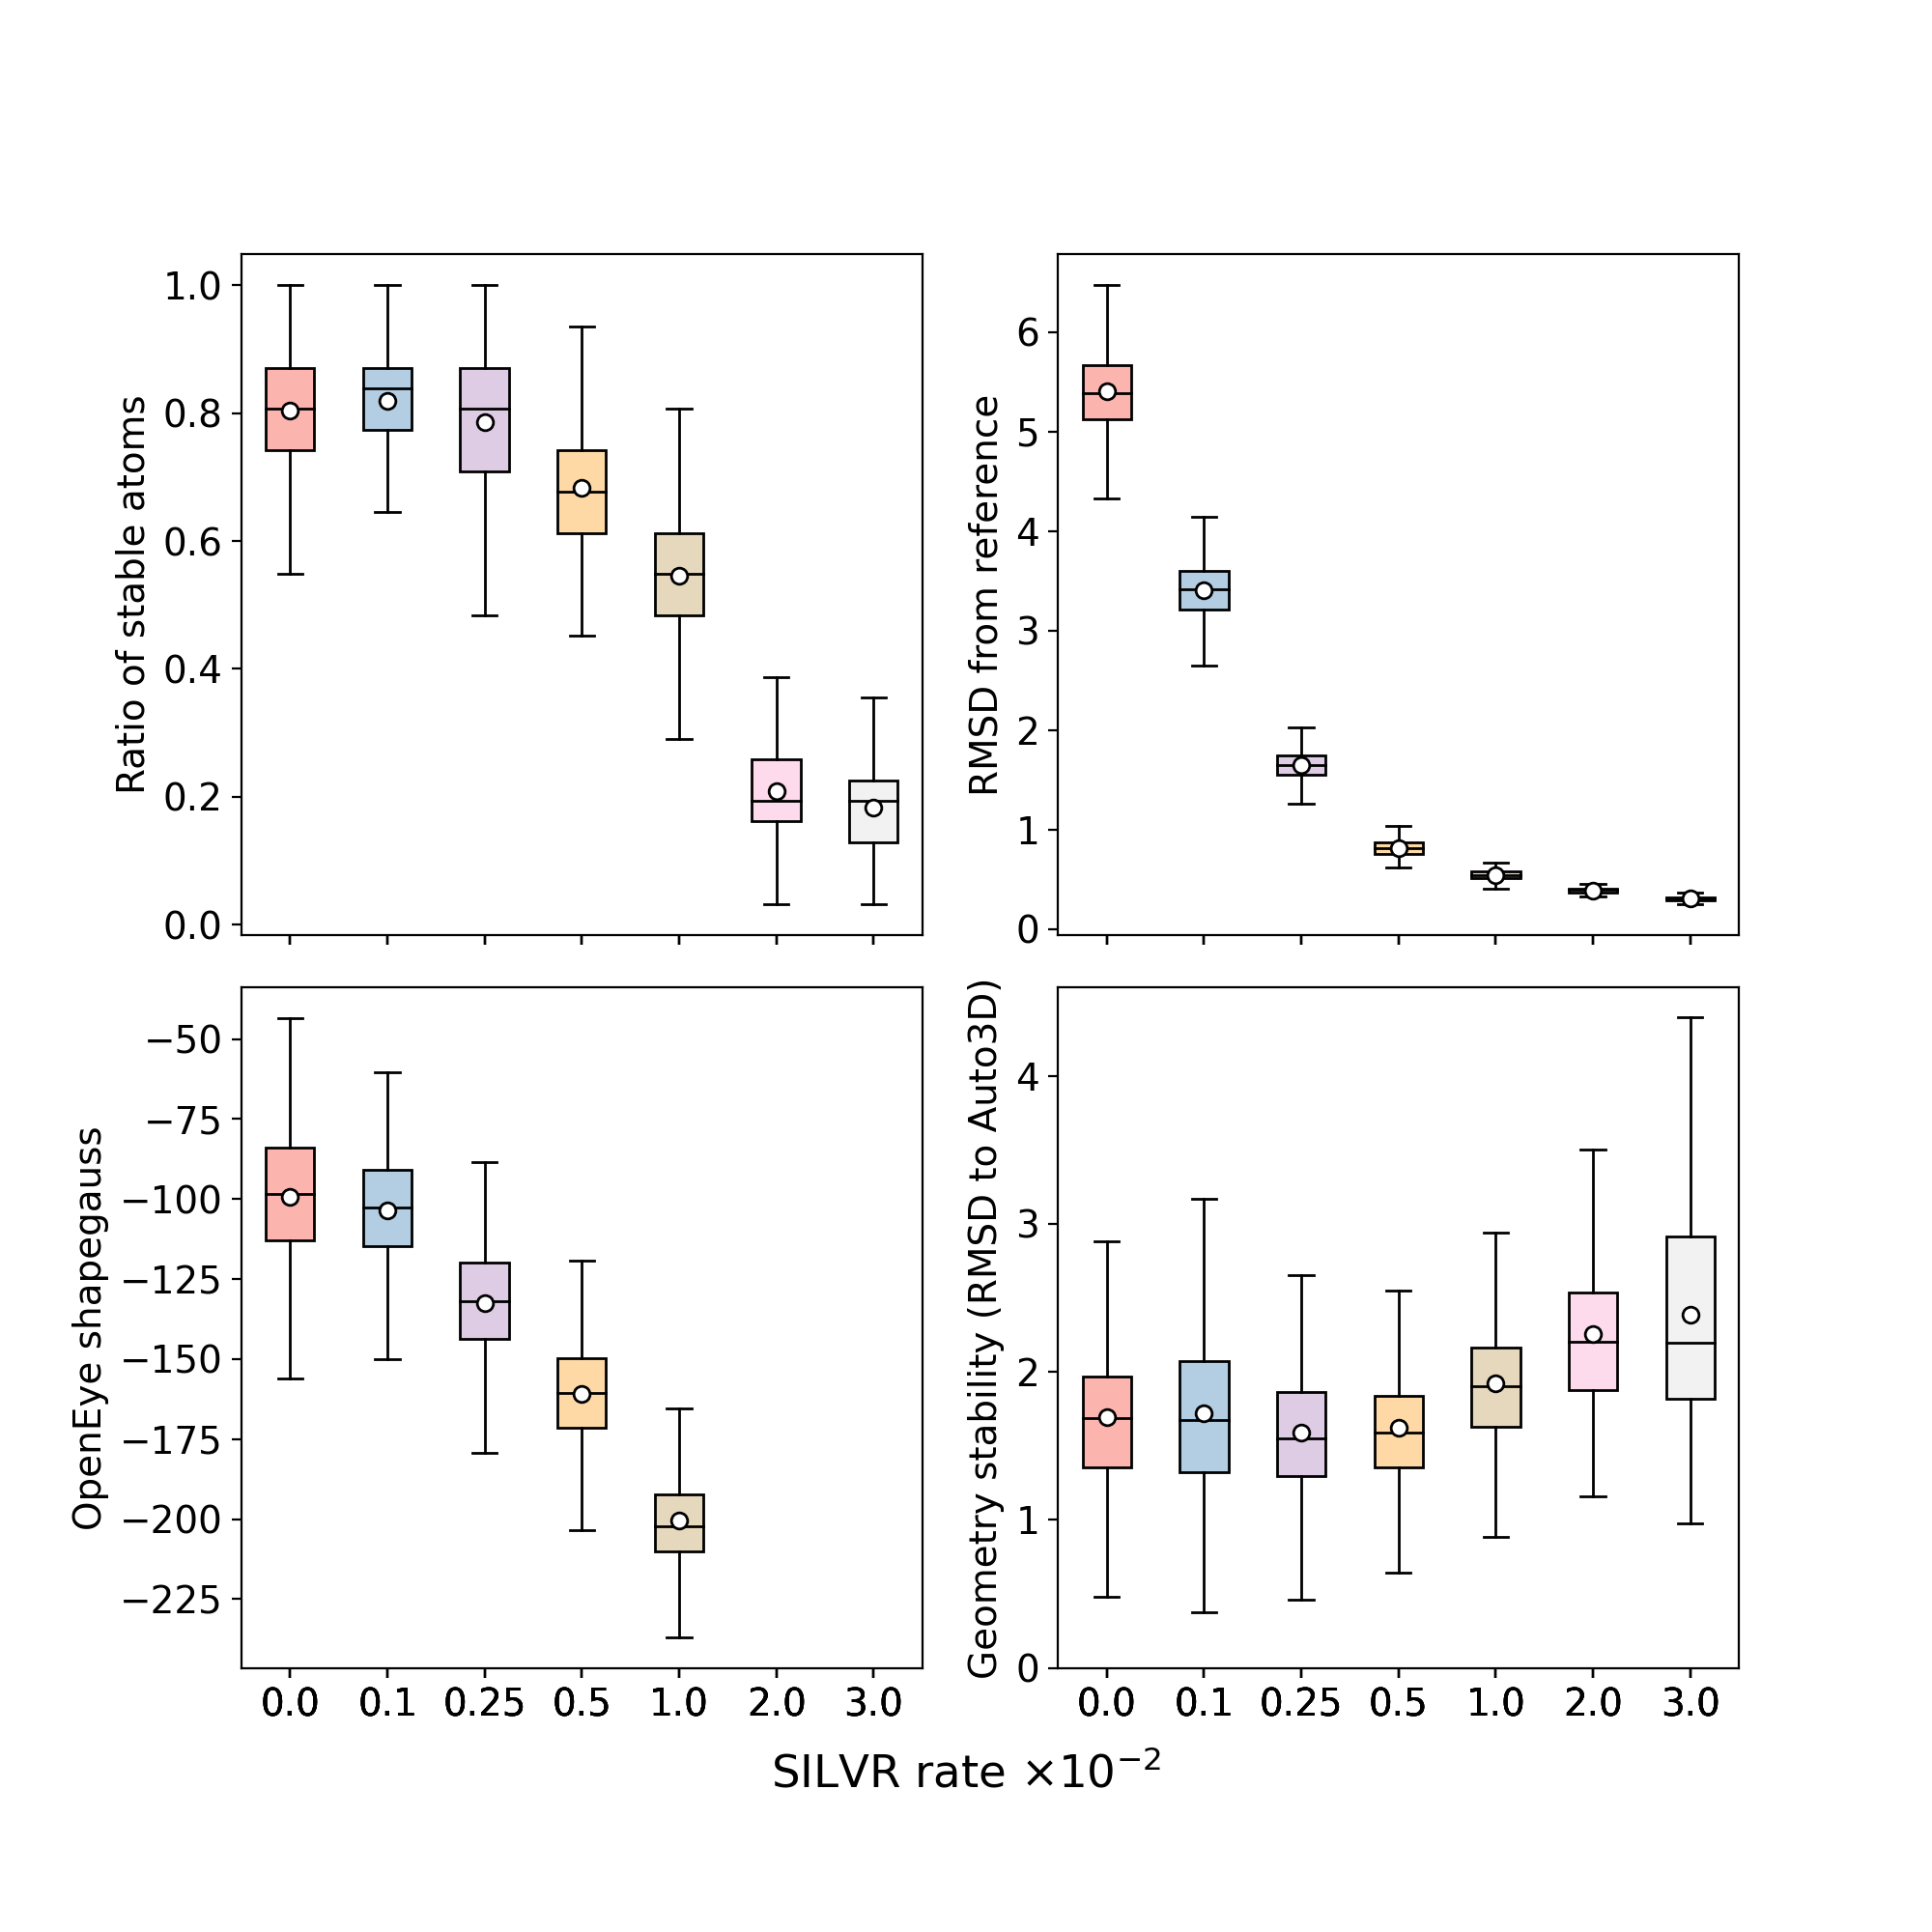
\includegraphics[width=\textwidth]{paper/Figures/Fig3/fig_3_metrics.png}
    \caption{Validation measures of SILVR model using fragments \texttt{x0072} and \texttt{x0354} as reference coordinates. A) Ratio of stable atoms - an atom is determined as stable if the valence matches the expected valence for the element B) RMSD from reference - the calculated RMSD between the reference and sample, using an absolute one-to-one mapping ignore atom identity C) OpenEye measure “shapegauss” - a Gaussian scoring function describing the shape fit between Mpro and samples, ignoring chemical interactions D) Geometry stability - AIMNet geometry optimisation was completed with Auto3D using the SMILES string of each sample. RMSD was calculated between the predicted geometry and the sampled geometry using RDKit.}
    \label{fig:measures}
\end{figure}
The similarity of samples to their reference set of coordinates was determined by RMSD, with a clear inverse correlation observed between rs and RMSD, as seen in Figure~\ref{fig:measures} b. This indicates that the extent of guidance of atoms towards the reference set of coordinates can be fine-tuned by varying $r_{\mathrm{S}}$. 

The next test we carried out was to determine whether the sampled molecular geometries are reasonable. For this purpose a separate geometry optimisation protocol was devised using the SMILES strings of the generated molecules and the RMSD between the generated molecule and the geometrically optimised molecule calculated. The results of this are found in Figure~\ref{fig:measures} d. At low to medium values of $r_{\mathrm{S}}$ ($< 0.01$), the average RMSD values all fall in the $1.6 - 1.7$ \AA~  range, which is arguably good, however still leaves sufficient room for improvement. Importantly, no difference is seen between the control set ($r_{\mathrm{S}}=0$) and the SILVR samples ($0 < r_{\mathrm{S}} < 0.01$) indicating the quality of generated molecules was not impeded by the SILVR protocol. 

\subsection{Generated samples with SILVR fit the binding site of Mpro}
As one of the main motivators for SILVR is to be able to generate new molecules that fit directly into a binding site based on input fragements, we measured shape complementarity between newly generated samples and the Mpro binding site. We used the OpenEye shapegauss scoring function for this purpose. From Figure~\ref{fig:measures} c it can be seen that the shape complementarity of samples improves with increasing $r_{\mathrm{S}}$, demonstrating that SILVR can produce ligands of binding site geometry when guided by the coordinates of fragment molecules. The lack of plot data for $r_{\mathrm{S}}=0.02$ and $r_{\mathrm{S}}=0.03$ was because all shapegauss calculations failed. We believe this was due to the atom coordinates representing highly strained and internally clashing molecules, and the scoring algorithm either failed to read the molecules or identified them as bad conformations.

\begin{figure}
    \centering
    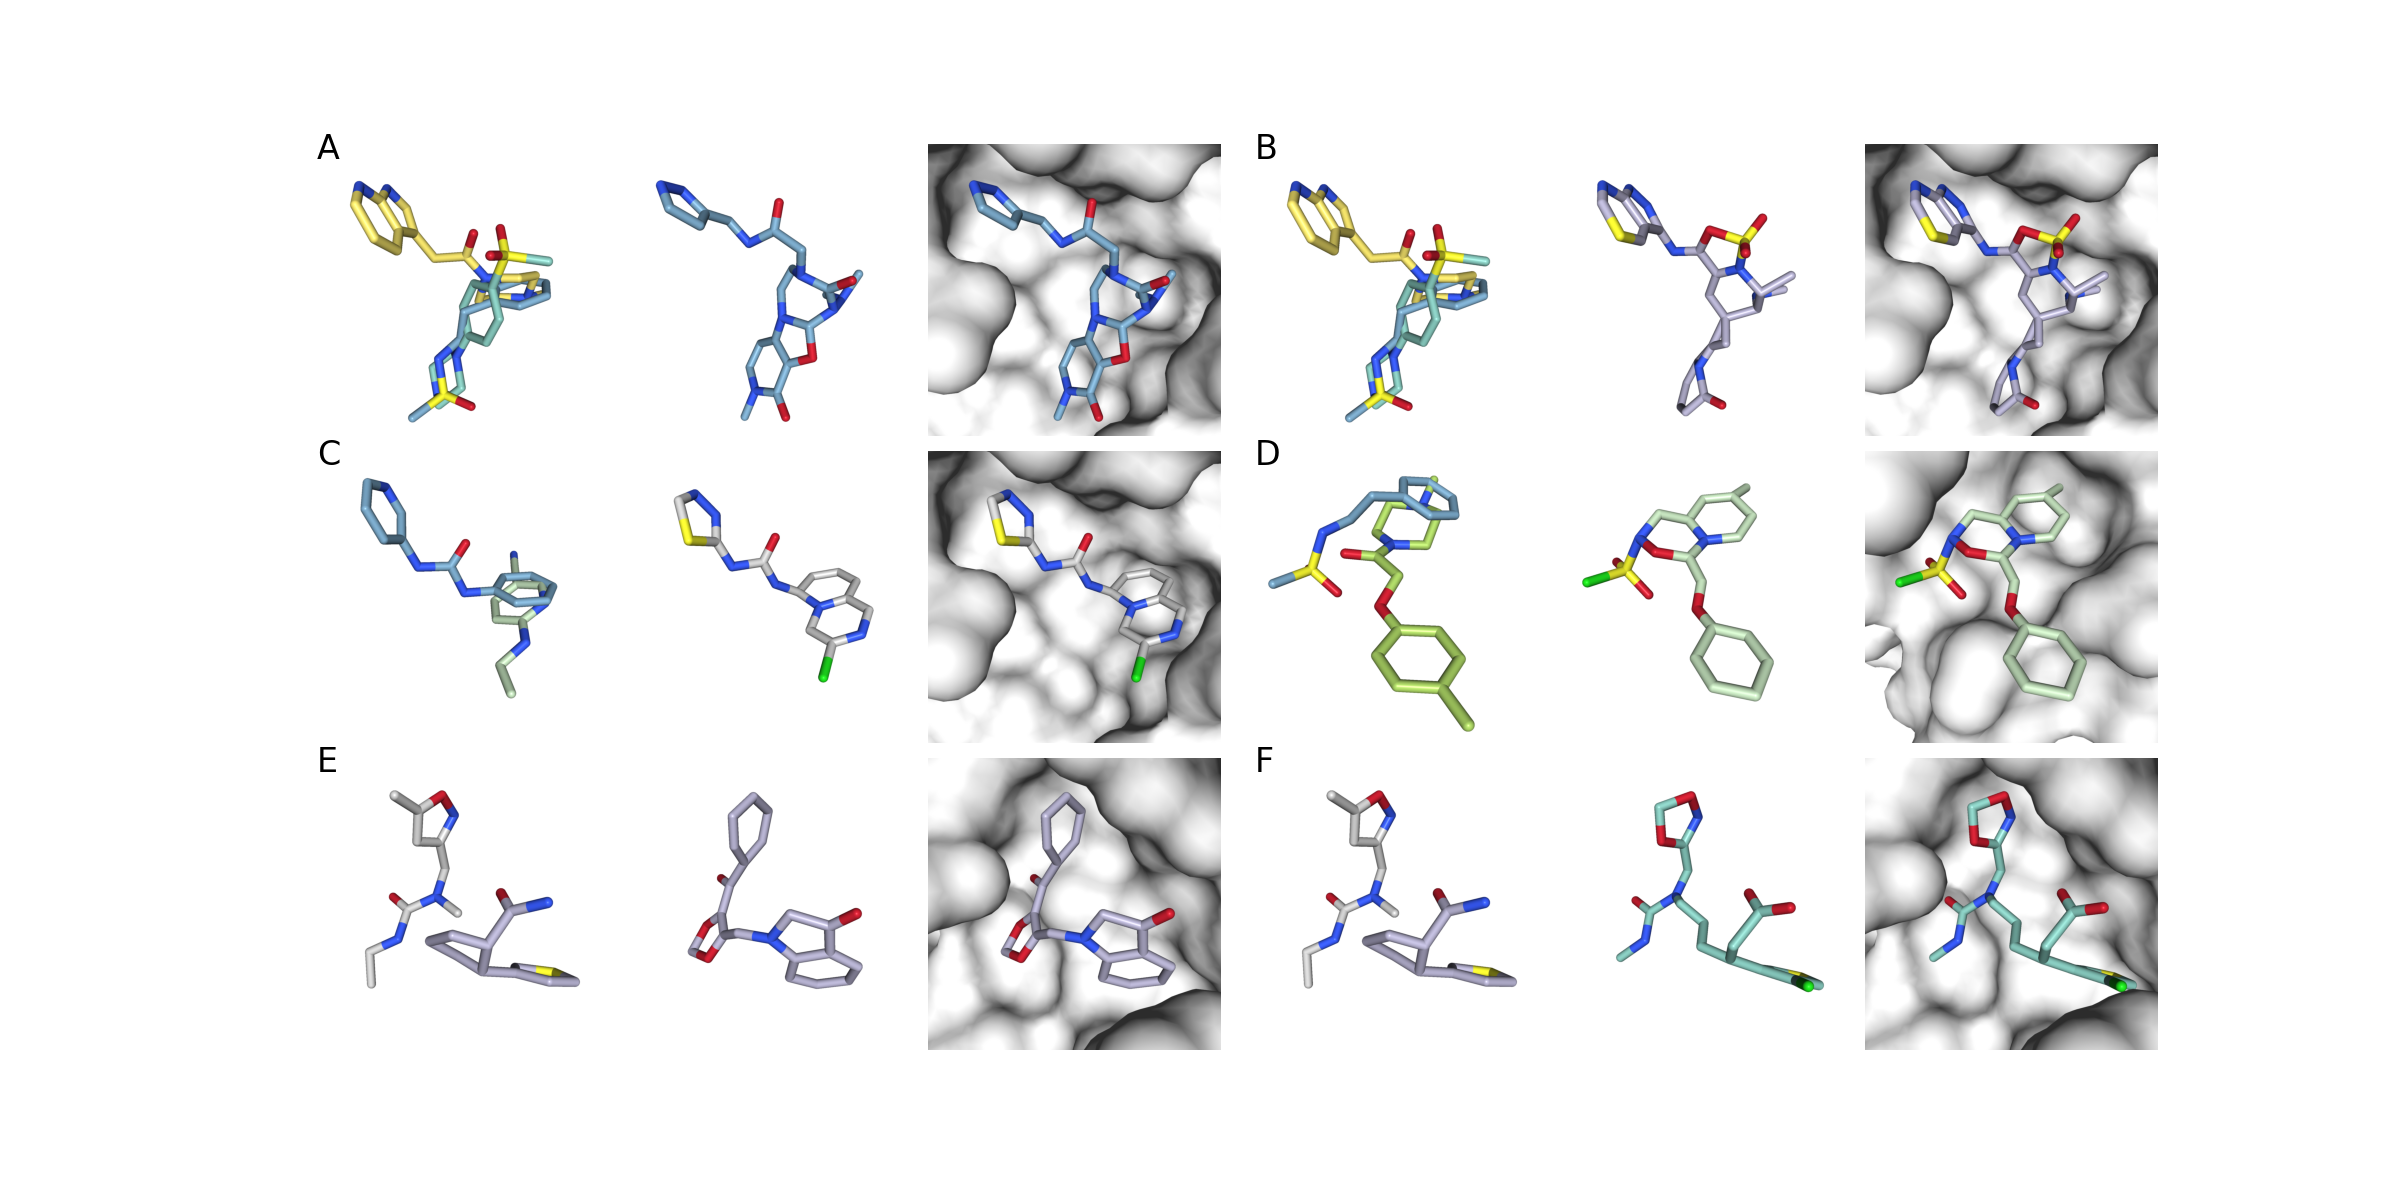
\includegraphics[width=\textwidth]{paper/Figures/Fig4/fig_4_ref_sample_bound.png}
    \caption{Examples of generated molecules from different experiments testing different overlap models. The reference fragments used as input to SILVR  are shown in the left column, the sampled molecule in the middle column, and the sampled molecule translated to the protein binding site in the right column. The left set of samples (A,C,E) has a SILVR rate $r_{\mathrm{S}}=0.005$, and the right set of samples (B, D, F) $r_{\mathrm{S}}=0.01$. Row 1: Three significantly overlapping fragments A and B (\texttt{x1093, x0072, x2193}). Row 2: Two fragments partially overlapping C (\texttt{x0434, x0305}), D (\texttt{x0072, x0354}). Row 3: Two disconnected fragments E and F (\texttt{x0874, x0397}) samples generated including 10 dummy atoms (method described in SI). The selection of molecules was hand-curated.}
    \label{fig:samples}
\end{figure}

In addition to the experiments using two fragments and generating 1000 samples, we also looked at different combinations of fragments and resulting molecules. In general, the trends of Figure~\ref{fig:measures} were preserved for all experiments with slight overall variations. Here we present three cases we investigated in detail.
\begin{enumerate}
    \item Using three fragments with substantial overlap as a reference.
    \item Using two fragments with a slight overlap. 
    \item Using two fragments that are disconnected to investigate linker generation. This scenario will be presented in detail in section~\ref{sec:linker}.
\end{enumerate}

Figure~\ref{fig:samples} A-F shows hand-curated samples for the 3 different scenarios for $r_{\mathrm{S}}=0.005$ (A,C,E) and $r_{\mathrm{S}}=0.01$ (B,D,F).

Figures~\ref{fig:samples}A and~\ref{fig:samples}B demonstrate a superposition of three significantly overlapping fragments that result in generated molecules that fit the Mpro binding site well. Scrutinising sample A with $r_{\mathrm{S}}=0.005$, we can see the azaindole fused ring system has been interpreted as a pyrrole ring, the ketone transformed into an amide (maintaining the same carbonyl position), the sulfonyl group vanished, and the overlapping atoms have transformed into a fused ring system. As a whole, the general geometry of the sample reflects the reference, however, functional groups are only weakly preserved. In contrast, sample B presents the same reference set but with $r_{\mathrm{S}}=0.01$. This new sample maintains the same geometry but better preserves key functional groups: the fused ring system is the same size, and satisfyingly the carbonyl oxygen has merged with the sulfonyl group to form a cyclic sulfamate ester.


Figure~\ref{fig:samples}C shows a merger of two partially overlapping fragments with $r_{\mathrm{S}}=0.005$. While the urea group was successfully preserved, the 6-membered ring shrank to a 5-membered heterocycle. Of particular interest is the formation of the fused ring system. At first glance, it might be assumed that reference atoms map to the sample atom closest in space, however in actuality they travel up to 1.7 \AA~to arrive at their final position (SI figure 4). In this case, the nitrogen atoms observed in the fused ring are directly obtained from the nitrogen atoms in the reference, however, their final position is one bond’s length from their reference. This shows the flexibility of each sample atom to explore within a radius (defined by $r_{\mathrm{S}}$) of the reference atom. The fact that the sample molecule populates a similar region of space to the reference is the result of the aggregate effects of each mapping, as opposed to the strict fixation of each atom. 

In contrast, Figure~\ref{fig:samples}D shows a stricter merging of two fragments, with $r_{\mathrm{S}}=0.01$. Visibly, the scaffold of the lower fragment has been maintained while the top fragment has contributed to a fused ring. Interestingly, the sulfonamide and carbonyl (from opposing fragments) have merged to form N-oxazinane sulfonyl chloride, demonstrating a particularly creative result from SILVR. 

\subsection{Fragments can be linked using SILVR and additional dummy atoms}
\label{sec:linker}
Being able to reliably link fragments that sit in a binding site of a protein is crucial for the design of potential new drugs. Being able to do so without retraining a model as was done by~\cite{huang20223dlinker}. Using conditioning through SILVR allows the generation of linkers between fragments without the need to retrain the EDM. This is illustrated in the example of Figure~\ref{fig:samples}E and F. While it was possible to use SILVR as described in the Theory section~\ref{sec:tehory}, better results were obtained with the addition of \textit{dummy atoms}. These are atoms which are present in the EDM without a mapping to a reference atom, and so are free to explore the whole coordinate space without guidance from SILVR. The successful implementation of dummy atoms requires a slight modification of the SILVR algorithm and is outlined in the SI. The results of these experiments continue the same trends previously observed where the $r_{\mathrm{S}}=0.005$ produces samples of approximate geometric similarity, whereas $r_{\mathrm{S}}=0.01$ produces a more strict mapping, with a clearly preserved urea group, a slightly modified ring system, and an amide interpreted as a carboxylate.

\section{Discussion and Outlook}
\label{sec:discussion}
SILVR, as presented, represents a promising proof of concept method in which a general EDM can be conditioned to generate samples that resemble a reference structure without any additional training needed. We could show that SILVR can complete both fragment merging and linking type tasks, without any \textit{a priori} knowledge of these design challenges. Considering all results with respect to the control EDM ($r_{\mathrm{S}}=0.0$), we show that at intermediate values of $r_{\mathrm{S}}$ the SILVR protocol produces molecules of equal quality to that of the unmodified EDM, while also guiding molecules towards reference structures. We, therefore, claim that if a diffusion model can be successfully trained to produce random high-quality drug-like structures, SILVR will provide molecular designs towards desired regions of chemical space without harming the quality of molecules. Our method poses a direct interface between crystallographic fragment data and \textit{de novo} molecular generation. However, there are a few ways in which the current method can be improved further but we deem out of scope for this work. 

\subsection{The number of unfragmented molecules generated can be improved}
The samples generated by SILVR are often of poorer quality than the samples selected in Figure~\ref{fig:samples}. Across all samples around half of the samples were determined by RDKit to be fragmented, meaning the sample contained two or more distinct molecular graphs. It was observed qualitatively that fragmented samples typically contained corrupted structures (multiple fragmentations, linear carbon chains, flattened rings, etc). We believe this fragmentation is triggered during intermediate steps of denoising, resulting in an unstable latent representation and subsequently poor EDM inference. Fragmentation becomes a particular issue for linker design type SILVR tasks (Figure~\ref{fig:samples}E and F), where the reference coordinates direct the latent variables away from each other, triggering fragmentation. For these experiments, 65\% of all samples were fragmented. Further work is needed both with EDM and with SILVR to reduce these rates of fragmentation. 

\subsection{The synthetic accessibility of the underlying EDM has a direct impact on the generated molecules}
 For our experiments, the synthetic accessibility of SILVR-generated molecules resembles the performance of the unmodified EDM. In order to achieve synthetically accessible samples with SILVR an improved EDM will need to be designed. An improved version of the EDM we have used has recently been proposed using more explicit information on bond order and represents the next appropriate step for testing SILVR~\cite{vignac2023midi}.

\subsection{There is no control over the retention of functional groups from the reference structure}
When applied to a drug design context, the conservation of key functional groups in exact spacial positions is crucial for the maintenance of protein-ligand interactions. The series of molecules in Figure S2 shows a loss of the sulfonyl chloride group present in the reference, which may be undesirable. This issue can be solved by changing $r_{\mathrm{S}}$ from a scalar to a vector ($\mathbf{r}_{\mathrm{S}}$), and by assigning particularly high $\mathbf{r}_{\mathrm{S}}$ values to selected atoms of the reference. Optimisation of $\mathbf{r}_{\mathrm{S}}$ vectors for actual drug design applications may become viable with a more suitably trained EDM.

\subsection{The inclusion of electrostatic information from proteins will likely improve the newly generated models}
To answer structure-based drug design, a scoring function of protein surface potentials could be used to guide atoms towards energetically favoured pocket regions; issues of synthetic accessibility might be solved by clever design of refinement methods; and interfacing with alternative data sources (such as NMR) might be achievable. 


\section{Conclusions}
We developed SILVR, a method that can be injected into a pre-trained equivariant diffusion model that serves as a molecular generator to explore new chemical space. SILVR allows the conditioning of molecules based on a reference set of molecules, e.g. a fragment from an X-ray fragment screen. The SILVR rate $r_{\mathrm{S}}$ allows the tuning of 'how much of the reference' molecule should be taken into account when generating new molecules, with medium values of $r_{\mathrm{S}}$ around 0.005 giving the best results. The simple conditioning against a reference set of molecules means that the model can be used for tasks of fragment linker design, as well as generating new molecules that fit into an existing binding pocket without any specific training needed towards these tasks. In the future, given improvements in EDMs that produce more realistic and synthetically accessible molecules this method can cheaply generate structures exploring new chemical space with desired conditioning towards existing fragment hits.

\section{Data Availability}
All data for the experiments carried out and instructions on how to reproduce this work can be found at~\url{https://github.com/meyresearch/SILVR}. An updated version of Hoogeboom et al. EDM that includes SILVR can be found at~\url{https://github.com/nichrun/e3_diffusion_for_molecules}.

%%%%%%%%%%%%%%%%%%%%%%%%%%%%%%%%%%%%%%%%%%%%%%%%%%%%%%%%%%%%%%%%%%%%%
%% The "Acknowledgement" section can be given in all manuscript
%% classes.  This should be given within the "acknowledgement"
%% environment, which will make the correct section or running title.
%%%%%%%%%%%%%%%%%%%%%%%%%%%%%%%%%%%%%%%%%%%%%%%%%%%%%%%%%%%%%%%%%%%%%
\begin{acknowledgement}
The authors thank Matteo T. Degiacomi and John D. Chodera for useful discussions and feedback on the manuscript. 
\end{acknowledgement}



%%%%%%%%%%%%%%%%%%%%%%%%%%%%%%%%%%%%%%%%%%%%%%%%%%%%%%%%%%%%%%%%%%%%%
%% The appropriate \bibliography command should be placed here.
%% Notice that the class file automatically sets \bibliographystyle
%% and also names the section correctly.
%%%%%%%%%%%%%%%%%%%%%%%%%%%%%%%%%%%%%%%%%%%%%%%%%%%%%%%%%%%%%%%%%%%%%
\bibliography{SILVR}

\end{document}